\documentclass[12pt,letterpaper]{article}
\usepackage{graphicx,textcomp}
\usepackage{natbib}
\usepackage{setspace}
\usepackage[a4paper,margin=1in]{geometry}
\usepackage{color}
\usepackage[reqno]{amsmath}
\usepackage{amsthm}
\usepackage{fancyvrb}
\usepackage{amssymb,enumerate}
\usepackage[all]{xy}
\usepackage{endnotes}
\usepackage{lscape}
\newtheorem{com}{Comment}
\usepackage{float}
\usepackage{hyperref}
\newtheorem{lem} {Lemma}
\newtheorem{prop}{Proposition}
\newtheorem{thm}{Theorem}
\newtheorem{defn}{Definition}
\newtheorem{cor}{Corollary}
\newtheorem{obs}{Observation}
\usepackage[compact]{titlesec}
\usepackage{dcolumn}
\usepackage{tikz}
\usetikzlibrary{arrows}
\usepackage{multirow}
\usepackage{xcolor}
\newcolumntype{.}{D{.}{.}{-1}}
\newcolumntype{d}[1]{D{.}{.}{#1}}
\definecolor{light-gray}{gray}{0.65}
\usepackage{url}
\usepackage{listings}
\usepackage{color}

\definecolor{codegreen}{rgb}{0,0.6,0}
\definecolor{codegray}{rgb}{0.5,0.5,0.5}
\definecolor{codepurple}{rgb}{0.58,0,0.82}
\definecolor{backcolour}{rgb}{0.95,0.95,0.92}

\lstdefinestyle{mystyle}{
	backgroundcolor=\color{backcolour},   
	commentstyle=\color{codegreen},
	keywordstyle=\color{magenta},
	numberstyle=\tiny\color{codegray},
	stringstyle=\color{codepurple},
	basicstyle=\footnotesize,
	breakatwhitespace=false,         
	breaklines=true,                 
	captionpos=b,                    
	keepspaces=true,                 
	numbers=left,                    
	numbersep=5pt,                  
	showspaces=false,                
	showstringspaces=false,
	showtabs=false,                  
	tabsize=2
}
\lstset{style=mystyle}
\newcommand{\Sref}[1]{Section~\ref{#1}}
\newtheorem{hyp}{Hypothesis}

\title{Problem Set 1}
\date{Due: October 9, 2025}
\author{Applied Stats/Quant Methods 1}

\begin{document}
	\maketitle
	
	\section*{Instructions}
	\begin{itemize}
	\item Please show your work! You may lose points by simply writing in the answer. If the problem requires you to execute commands in \texttt{R}, please include the code you used to get your answers. Please also include the \texttt{.R} file that contains your code. If you are not sure if work needs to be shown for a particular problem, please ask.
\item Your homework should be submitted electronically on GitHub.
\item This problem set is due before 23:59 on Thursday October 9, 2025. No late assignments will be accepted.
	\end{itemize}
	
	\vspace{1cm}
	\section*{Question 1: Education}

A school counselor was curious about the average of IQ of the students in her school and took a random sample of 25 students' IQ scores. The following is the data set:\\
\vspace{.5cm}

\lstinputlisting[language=R, firstline=36, lastline=36]{PS01_DP.R}  

\vspace{1cm}

\begin{enumerate}
	\item Find a 90\% confidence interval for the average student IQ in the school.\\
	
	\item Next, the school counselor was curious  whether  the average student IQ in her school is higher than the average IQ score (100) among all the schools in the country.\\ 
	
	\noindent Using the same sample, conduct the appropriate hypothesis test with $\alpha=0.05$.
\end{enumerate}

\newpage
	\section*{Solution - Question 1: Education}
\vspace{.5cm}
\subsection*{1. Confidence Interval for the Average Student IQ in the School} 
\vspace{.5cm}
Since the sampling size is smaller than 30, we cannot assume that there is a normal sampling distribution. Instead, we will assume a t-distribution with 25-1 = 24 degrees of freedom (because the sample has n = 25 observations). \\[0.5cm]
The process for determining the confidence interval is outlined below: 
\begin{itemize}
	\item 
	Calculate the mean 
	\lstinputlisting[language=R, firstline=39, lastline=40]{PS01_DP.R} 
  \begin{verbatim}
  	[1] 98.44
  \end{verbatim}
  \item 
  Calculate the sum of the squared errors to get the variance, and then the  standard deviation (the square root of the variance)
  	\lstinputlisting[language=R, firstline=43, lastline=47]{PS01_DP.R} 
  \begin{verbatim}
  	[1] 13.09287
  \end{verbatim}
  \item 
  Calculate the standard error 
  \lstinputlisting[language=R, firstline=50, lastline=51]{PS01_DP.R} 
  \begin{verbatim}
  	[1] 2.618575
  \end{verbatim}
   \item 
  Find the t-score for the desired confidence level, with 24 degrees of freedom \\
  I calculated the t-score instead of a Z-score because the assumed sampling distribution is a t-distribution with 24 degrees of freedom. 
  \lstinputlisting[language=R, firstline=54, lastline=55]{PS01_DP.R} 
  \begin{verbatim}
  	[1] 1.710882
  \end{verbatim}
  \newpage
   \item 
  Construct the confidence interval by calculating its lower and upper limits
  \lstinputlisting[language=R, firstline=58, lastline=61]{PS01_DP.R} 
  \begin{verbatim}
  	> lowerlimit
  	[1] 93.95993
  	> upperlimit
  	[1] 102.9201
  \end{verbatim}
  \item 
  \textbf{Conclusion:} The interval [93.96, 102.92] contains the true average of student IQs at the school (the true population mean) at least 90\% of the time, with repeated random sampling.  
  \end{itemize}
\vspace{1cm}
\subsection*{2. Hypothesis Testing}\\
\vspace{.5cm}
\begin{itemize}
	\item \underline{\textbf{Step 1:} assumptions}\\
	\begin{itemize}
		\item the data is quantitative and continuous 
		\item the sampling method is random
		\item the sample size is smaller than 30, so we assume it follows a t-distribution with 24 degrees of freedom and not a normal distribution; the test statistic that was calculated is a t-score 
	\end{itemize}
	\item \underline{\textbf{Step 2:} formulate hypotheses}\\
	\begin{itemize}
		\item \textbf{Null hypothesis:} the average student IQ in the school (the mean) is lower than or equal to 100 
		\item \textbf{Alternative hypothesis:} the average student IQ in the school (the mean) is higher than 100 
	\end{itemize}
	\item \underline{\textbf{Step 3: } calculate the test statistic : t-score}\\
		\lstinputlisting[language=R, firstline=70, lastline=71]{PS01_DP.R} 
		\begin{verbatim}
			[1] -0.5957439
		\end{verbatim}
\newpage
	\item \underline{\textbf{Step 4:} calculate the p-value}\\[0.5cm]
	Because the hypothesis test that is carried out is one-sided, and the alternative hypothesis is that the true population mean is greater than 100, we are interested in the upper tail of the distribution. Hence, the lower.tail argument was set to FALSE.
\lstinputlisting[language=R, firstline=74, lastline=75]{PS01_DP.R} 
	\begin{verbatim}
		[1] 0.7215383
	\end{verbatim}
	\item\underline{\textbf{Step 5:} draw a conclusion}\\[0.5cm]
	The p-value is much higher than the alpha value (0.05). Thus, we cannot reject the null hypothesis that the average student IQ in the school is lower than or equal to 100. The test result is not statistically significant. 
\end{itemize}

\newpage
	\section*{Question 2: Political Economy}

\noindent Researchers are curious about what affects the amount of money communities spend on addressing homelessness. The following variables constitute our data set about social welfare expenditures in the USA. \\
\vspace{.5cm}


\begin{tabular}{r|l}
	\texttt{State} &\emph{50 states in US} \\
	\texttt{Y} & \emph{per capita expenditure on shelters/housing assistance in state}\\
	\texttt{X1} &\emph{per capita personal income in state} \\
	\texttt{X2} &  \emph{Number of residents per 100,000 that are "financially insecure" in state}\\
	\texttt{X3} &  \emph{Number of people per thousand residing in urban areas in state} \\
	\texttt{Region} &  \emph{1=Northeast, 2= North Central, 3= South, 4=West} \\
\end{tabular}

\vspace{.5cm}
\noindent Explore the \texttt{expenditure} data set and import data into \texttt{R}.
\vspace{.5cm}
\lstinputlisting[language=R, firstline=6, lastline=6]{PS01_DP.R}  
\vspace{.5cm}
\begin{itemize}

\item
Please plot the relationships among \emph{Y}, \emph{X1}, \emph{X2}, and \emph{X3}? What are the correlations among them (you just need to describe the graph and the relationships among them)?
\vspace{.5cm}
\item
Please plot the relationship between \emph{Y} and \emph{Region}? On average, which region has the highest per capita expenditure on housing assistance?
\vspace{.5cm}
\item
Please plot the relationship between \emph{Y} and \emph{X1}? Describe this graph and the relationship. Reproduce the above graph including one more variable \emph{Region} and display different regions with different types of symbols and colors.
\end{itemize}
\newpage
	\section*{Solution - Question 2: Political Economy}
	\subsection*{Plot the relationships among X1, X2, X3 and Y}
\lstinputlisting[language=R, firstline=96, lastline=103]{PS01_DP.R} 
\vspace{.5cm}
\begin{figure}[h!]\centering
	\caption{\footnotesize Scatterplot of X1 and Y}
	\label{fig:plot_1}
	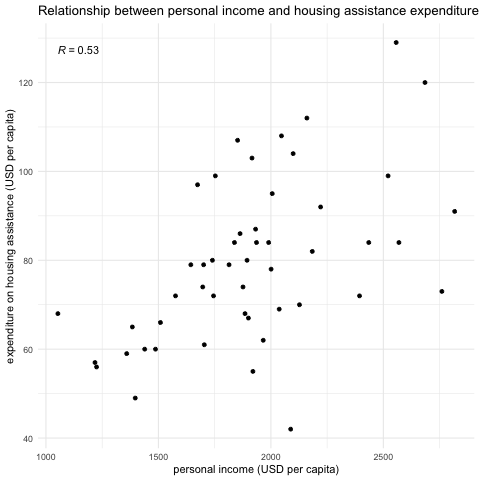
\includegraphics[width=.7\textwidth]{scatter_x1_y.png}
\end{figure} 
\vspace{.5cm}
\underline{\textbf{Interpretation:}}\\[.3cm]There is a moderate positive association between the personal income and the expenditure on housing assistance per capita in a state. The Pearson correlation coefficient points towards the same conclusion, as its value is above 0, but not close enough to 1 to suggest a strong association between the two variables. A positive linear pattern can also be distinguished by looking at the plot. 
\newpage
\lstinputlisting[language=R, firstline=107, lastline=114]{PS01_DP.R} 
\vspace{.5cm}
\begin{figure}[h!]\centering
	\caption{\footnotesize Scatterplot of X2 and Y}
	\label{fig:plot_2}
	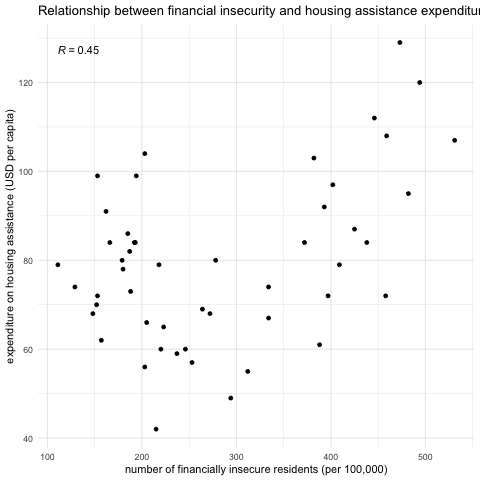
\includegraphics[width=.7\textwidth]{scatter_x2_y.png}
\end{figure}
\vspace{.5cm}
\underline{\textbf{Interpretation:}}\\[.3cm] There is a moderate positive association between the number of "financially insecure" residents and the expenditure on housing assistance per capita in a state. The Pearson correlation coefficient suggests the same, as its value is above 0, but not above 0.5. Visually analysing the plot, there is an upward linear trend that can be identified, but there are many dots that fall outside of it, which suggests that the association is fairly weak. 
\newpage
\lstinputlisting[language=R, firstline=118, lastline=125]{PS01_DP.R} 
\vspace{.5cm}
\begin{figure}[h!]\centering
	\caption{\footnotesize Scatterplot of X3 and Y}
	\label{fig:plot_3}
	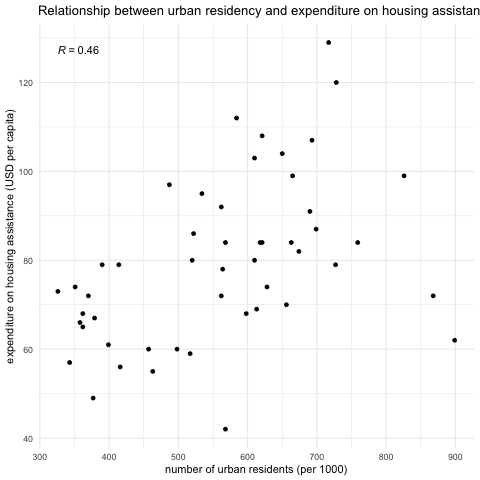
\includegraphics[width=.7\textwidth]{scatter_x3_y.png}
\end{figure}
\vspace{.5cm}
\underline{\textbf{Interpretation:}}\\[.3cm] There is a mild positive association also between the number of residents in urban areas and the expenditure on housing assistance per capita in a state. The value of the Pearson correlation coefficient is 0.46, suggesting a weak association between the two variables. There is a faint upward linear trend that can be observed from the plot, but the dots are very loosely grouped around it. 
\newpage
\lstinputlisting[language=R, firstline=129, lastline=136]{PS01_DP.R} 
\vspace{.5cm}
\begin{figure}[h!]\centering
	\caption{\footnotesize Scatterplot of X1 and X2}
	\label{fig:plot_4}
	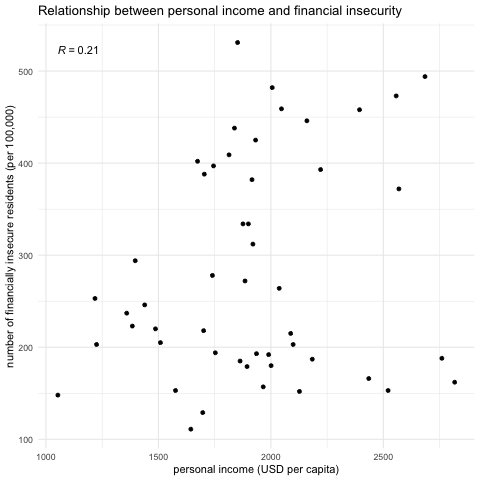
\includegraphics[width=.7\textwidth]{scatter_x1_x2.png}
\end{figure}
\vspace{.5cm}
\underline{\textbf{Interpretation:}}\\[.3cm] There doesn't seem to be a linear association between personal income per capita and the number of "financially insecure" residents within a state. The data points appear to be quite scattered in the graph, showing no clear linear trend. The Pearson correlation coefficient has a value of 0.21, indicating that we can only observe a very weak, if any, association between the two variables.
\newpage
\lstinputlisting[language=R, firstline=140, lastline=147]{PS01_DP.R} 
\vspace{.5cm}
\begin{figure}[h!]\centering
	\caption{\footnotesize Scatterplot of X1 and X3}
	\label{fig:plot_5}
	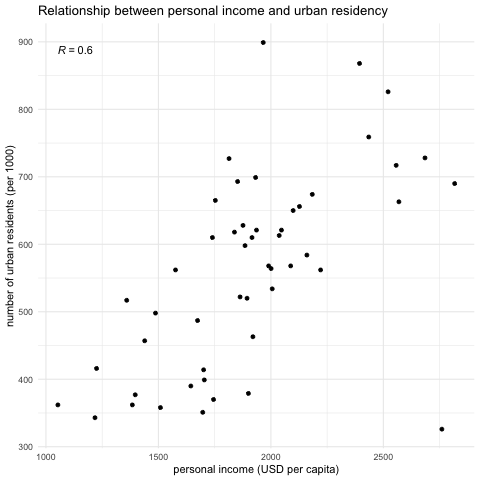
\includegraphics[width=.7\textwidth]{scatter_x1_x3.png}
\end{figure}
\vspace{.5cm}
\underline{\textbf{Interpretation:}}\\[.3cm] There is a moderate positive association between the personal income per capita and the number of urban residents in a state. The value of the Pearson correlation coefficient shows that these two variables have the strongest correlation within the dataset, but the value is still not high enough to indicate a strong association. Visually inspecting the plot, it can be observed that the dots follow an upward linear trend, but they are not very tightly grouped around it. 
\newpage
\lstinputlisting[language=R, firstline=151, lastline=158]{PS01_DP.R} 
\vspace{.5cm}
\begin{figure}[h!]\centering
	\caption{\footnotesize Scatterplot of X2 and X3}
	\label{fig:plot_6}
	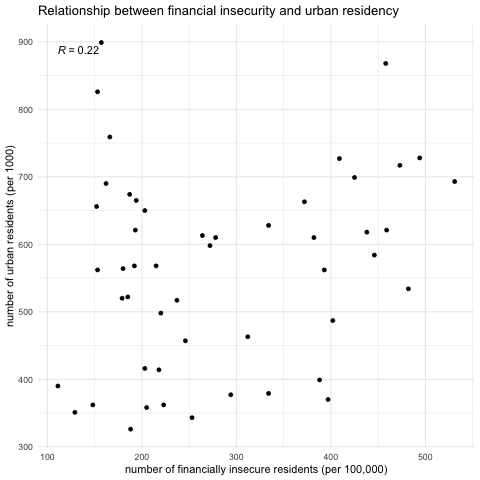
\includegraphics[width=.7\textwidth]{scatter_x2_x3.png}
\end{figure}
\vspace{.5cm}
\underline{\textbf{Interpretation:}}\\[.3cm] There doesn't seem to be a linear association between the number of "financially insecure" residents and the number of urban residents in a state. The dots are spread out quite evenly within the plot, without any distinguishable pattern. The Pearson correlation coefficient is quite close to 0, further indicating the absence of a meaningful association between the two variables. 
\newpage
\subsection*{Plot the relationship between Y and Region}
\lstinputlisting[language=R, firstline=170, lastline=178]{PS01_DP.R} 
\vspace{.5cm}
\begin{figure}[h!]\centering
	\caption{\footnotesize Boxplot of Y and Region}
	\label{fig:plot_7}
	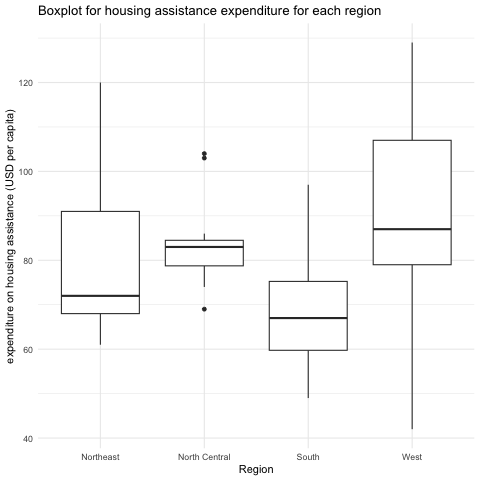
\includegraphics[width=.7\textwidth]{boxplot_reg_y.png}
\end{figure}
\vspace{.5cm}
\underline{\textbf{Interpretation:}}\\[.3cm] In order to visualize the average expenditure on housing assistance in each region, I generated a boxplot. This type of plot was chosen because it shows the distribution of data for each region, indicating the median but also the variability of the values. \\ It can be observed that the West region has the highest median for expenditure on housing assistance per capita and its interquartile range starts and ends at higher values than the others. Thus, the West spends on average the most out of the regions to provide housing assistance. 
\newpage
\subsection*{Plot the relationship between Y, X1 and Region }
\lstinputlisting[language=R, firstline=184, lastline=195]{PS01_DP.R} 
\vspace{.5cm}
\begin{figure}[h!]\centering
	\caption{\footnotesize Scatterplot of X1, Y and Region}
	\label{fig:plot_8}
	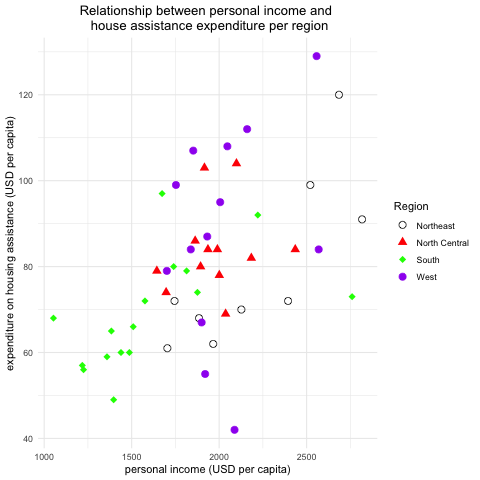
\includegraphics[width=.7\textwidth]{scatter_x1_y_reg.png}
\end{figure}
\vspace{.5cm}
\underline{\textbf{Interpretation:}}\\[.3cm] In the previous plot of personal income and expenditure on housing assistance per capita in a state (Figure 1), a moderate positive association between the two was identified. This plot highlighting the values from different regions adds a new layer of interpretation. \\ Most notably, the South region shows on average both low income and low expenditure on housing assistace. The North Central region seems to also have mostly values for personal income that are proportional with the expenditure on housing assistance, the observations being concetrated towards the centre of the plot. Nevertheless, the West region shows some contrast in terms of expenditure on housing assistance for similar personal income values. This suggests that factors at the regional level might be correlated with both the housing assistance expenditure and the personal income per capita, and the association between the two of them might require further consideration and assessment. 
\end{document}

